
\documentclass[a4paper,12pt,oneside,pdflatex,italian,final,twocolumn]{article}

\usepackage[utf8]{inputenc}
\usepackage{parallel}
\usepackage{siunitx}
\usepackage{booktabs}
\usepackage{fancyhdr}
\usepackage{subcaption}
\usepackage{listings}

\usepackage[export]{adjustbox}
\usepackage[margin=0.5in]{geometry}
\addtolength{\topmargin}{0in}

\usepackage{libertine}
\renewcommand*\familydefault{\sfdefault}  %% Only if the base font of the document is to be sans serif
\usepackage[T1]{fontenc}







\title{ElbiCare Audiometri}
\author{Achmadi ST MT}
\date{August 2022}

\begin{document}

\pagestyle{fancy}

\lhead{VibrasticLab}
\chead {\today}
\rhead{Specification Document v1.0}


\onecolumn

\begin{figure}
\begin{minipage}{0.47\textwidth}
\centering

\end{minipage}
\hfill
\begin{minipage}{0.47\textwidth}
\raggedleft
\Huge \textbf{Portable Audiometri v3.0}
\end{minipage}
\end{figure}


\begin{figure}
\begin{minipage}{0.47\textwidth}

\section{Overview}
    \begin{itemize}
        \item Standardized 3-Force Choice Method
        \item Fast hearing screening
        \item Portable handheld
        \item Cloud connected
        \item Easy to use
    \end{itemize}


\end{minipage}
\hfill
\begin{minipage}{0.47\textwidth}
\centering
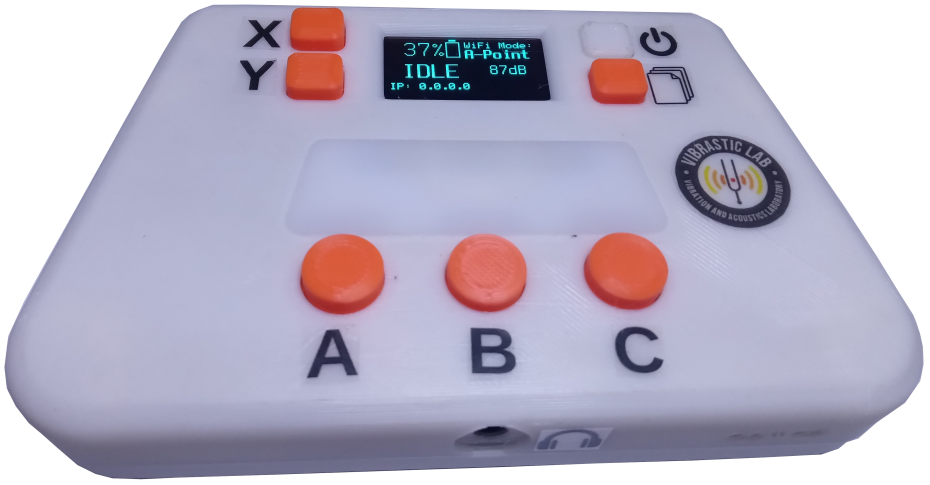
\includegraphics[width=0.7\textwidth,right]{images/audiometri.png}

\end{minipage}
\end{figure}



\section{Description}
\begin{itemize}

\item Hearing screening using 3-Force Choice Method to minimize biased results

\item Each screening session approximately can be done in roughly 10 minutes.

\item Battery operated apparatus with very ergonomic handheld design

\item Screening results stored locally on Micro-SD Card and can also be uploaded to cloud-storage for futher analysis and longer-term record.

\item No need complex settings and can be used right away.

\item Equipped with embbedded MEMS microphone for boothless usage.

\item Easy to maintenance without any disassembly process required.

\end{itemize}

\section{Technical specification}
\centering
\begin{tabular}{lcr}
\toprule
Parts & Unit & Value \\
\midrule
Power voltage & $V$ & 5 \\
Dimensions & $mm*mm*mm$ & xx*yy*zz (without cable) \\
Weight & $g$ & x \\
Network & & IEEE 802.11b/g/n 2.4GHz \\
Storage & & Micro-SD Slot \\
Audio Port & & 3.5mm TRS \\
USB  Data Interface & & USB-CDC Serial \\
\bottomrule
\end{tabular}

\raggedright

\section{Measured Output Tone}

\centering
\begin{tabular}{lcr}
\toprule
  Frequency & Tone Range(*) \\
\midrule
250 Hz & 17-55 dBA \\
500 Hz & 20-60 dBA \\
1000 Hz & 31-68 dBA \\
2000 Hz & 28-64 dBA \\
4000 Hz & 42-80 dBA \\
6000 Hz & 33-72 dBA \\
\bottomrule
\end{tabular}

\vspace{5pt}
\footnotesize{(*): Tested on JBL T500 headphone unit}



\raggedright
\section{User Interfaces}
\centering
\begin{figure} [h]
\centering
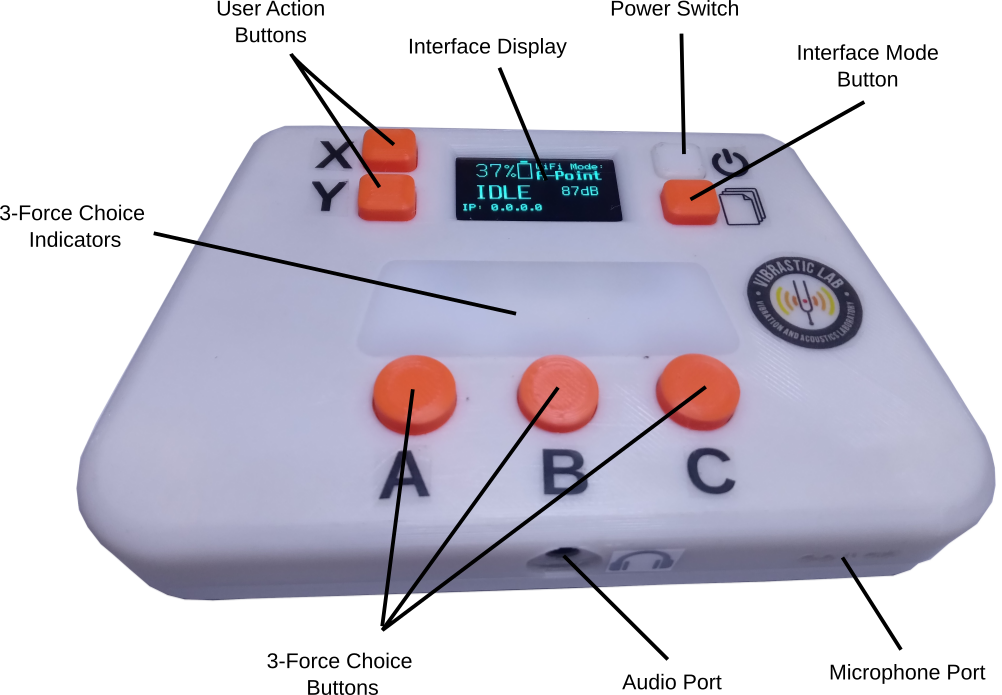
\includegraphics[width=0.55\textwidth,]{images/useriface.png}
\caption{General User Interface and Features}
\end{figure}

\begin{figure} [h]
\centering
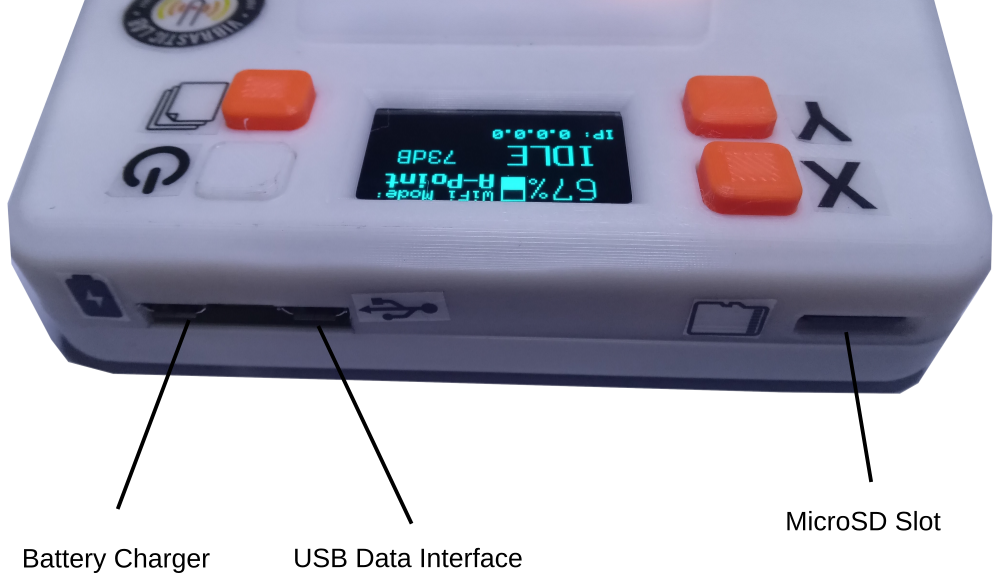
\includegraphics[width=0.55\textwidth,]{images/portuser.png}
\caption{Data and Power Ports}
\end{figure}

\raggedright
\subsection{User Mode Button selection}

\begin{figure}[h]
    \centering
    \begin{subfigure}[b]{0.32\textwidth}
        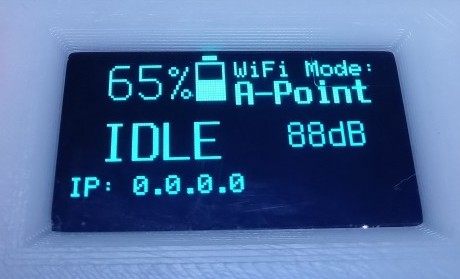
\includegraphics[width=\textwidth]{images/display-home.jpg}
        \caption{Home Display}
    \end{subfigure}
    ~
    \begin{subfigure}[b]{0.32\textwidth}
        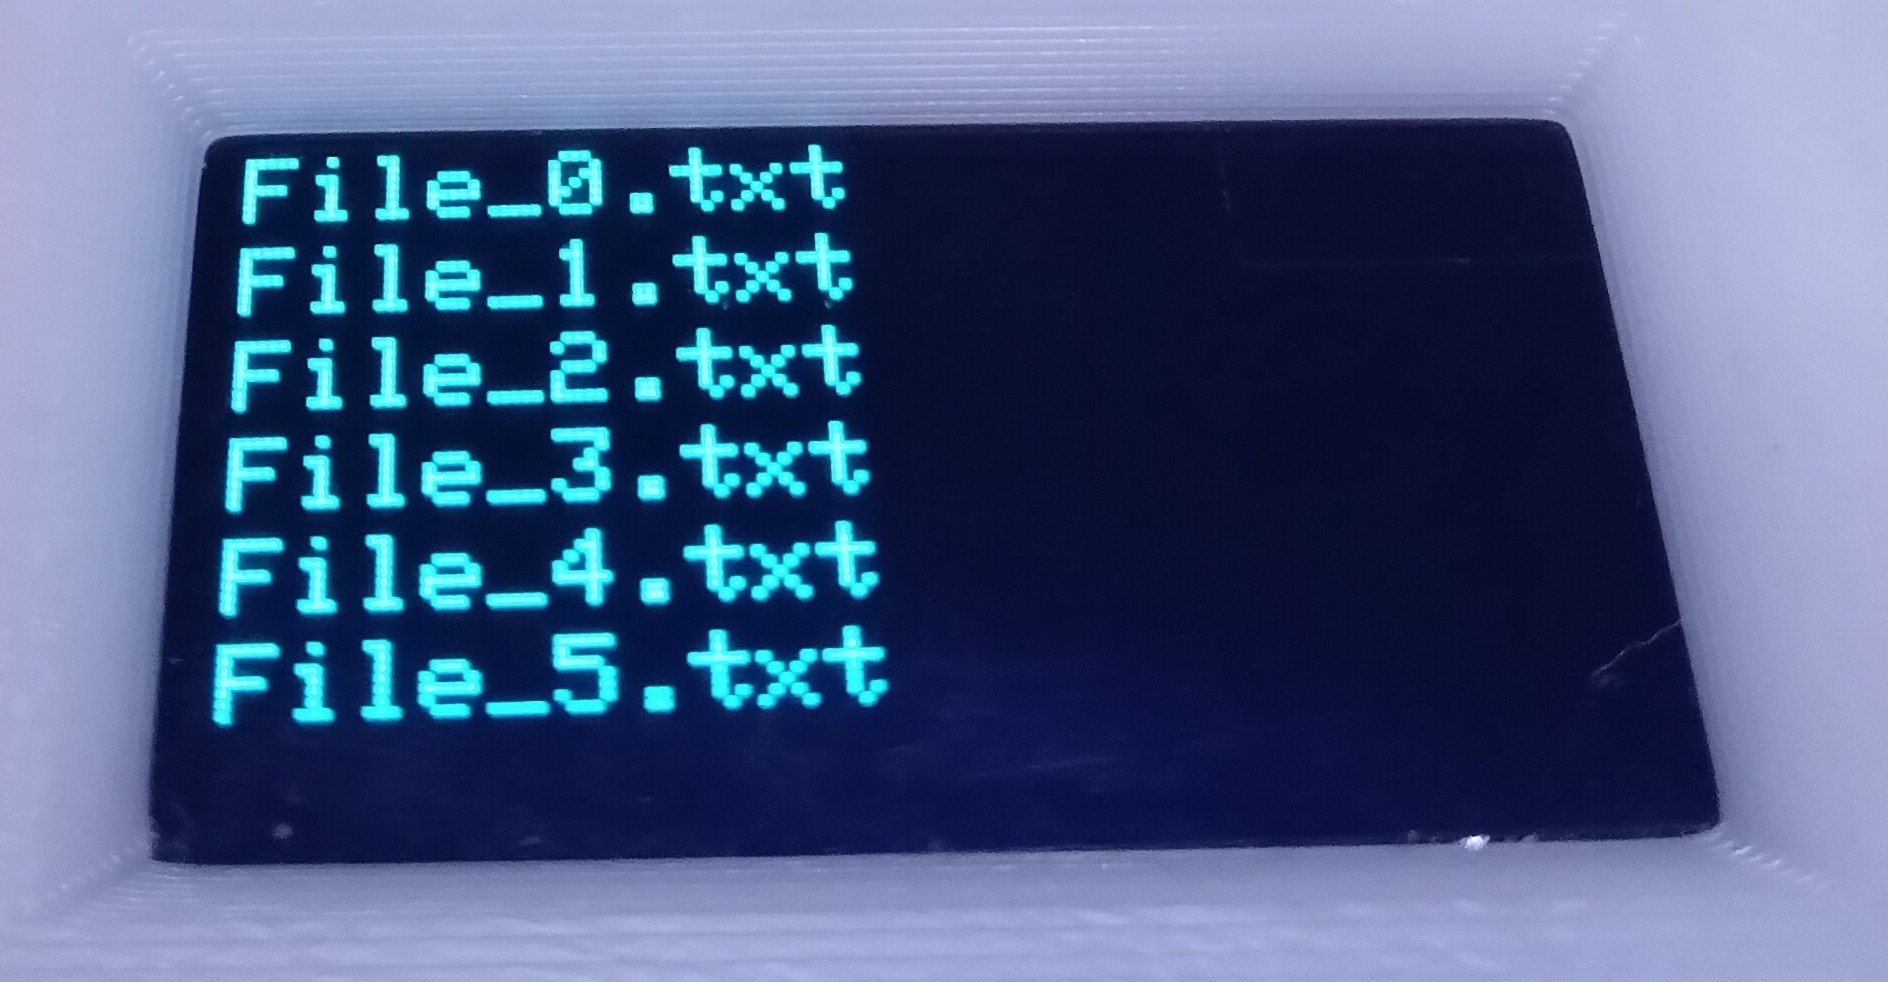
\includegraphics[width=\textwidth]{images/display-file.jpg}
        \caption{File List}
    \end{subfigure}
    ~
    \begin{subfigure}[b]{0.32\textwidth}
        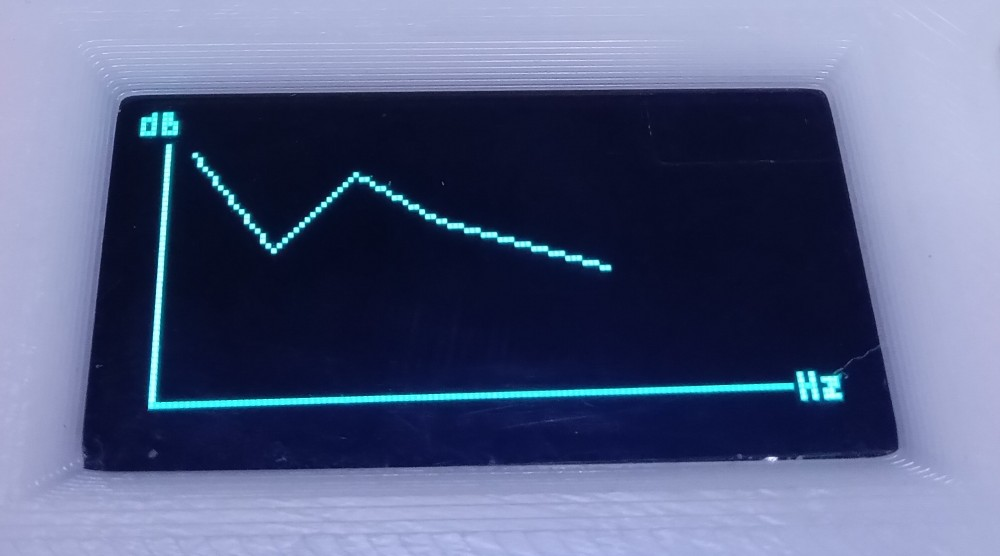
\includegraphics[width=\textwidth]{images/display-plot.jpg}
        \caption{Audiogram Preview}
    \end{subfigure}
\end{figure}

\newpage
\raggedright
\section{3-Force Choice}

\subsection{Starting}

\begin{figure} [h]
    \centering
    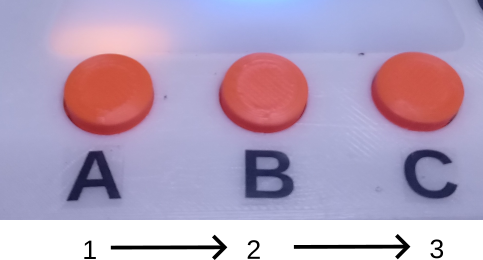
\includegraphics[width=0.4\textwidth,]{images/3fc_start.png}
    \caption{Starting screening session buy press 3-Force Buttons sequentially}
\end{figure}

\subsection{Answering}

\begin{figure} [h]
    \centering
    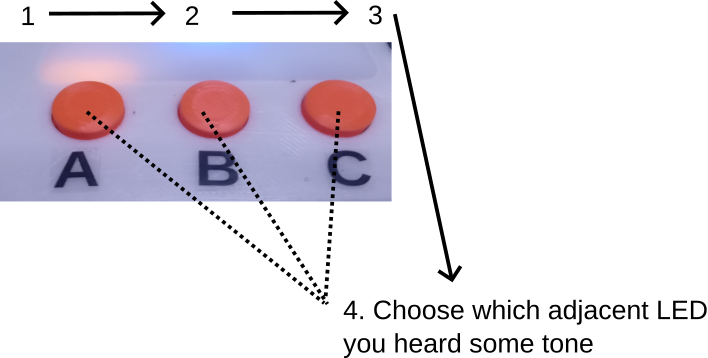
\includegraphics[width=0.7\textwidth,]{images/3fc_answer.png}
    \caption{Answering 3-Force Choice by pressing button adjacent to a LED which light-up when a tone has been heard}
\end{figure}

\raggedright
\section{Charging}

\begin{figure} [h]
    \centering
    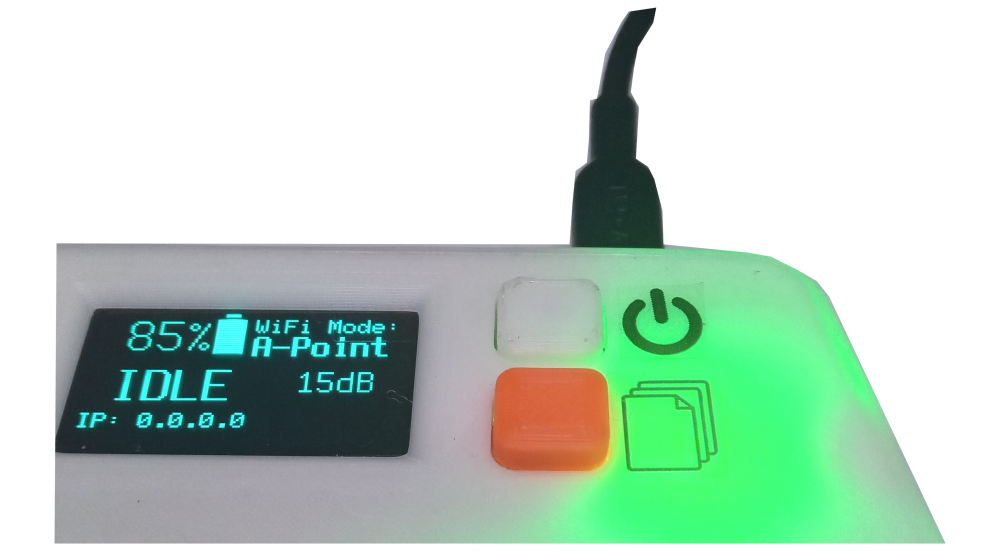
\includegraphics[width=0.4\textwidth,]{images/charging.png}
    \caption{Operated on rechargeable battery (please do not charging while using the apparatus)}
\end{figure}

\newpage
\raggedright
\section{Screening Result Determination}

Example of internal Micro-SD card record file:

\begin{lstlisting}
{"audiogram":{

"ch_0":{
"freq_0":{"freq": 0.625,"ampl":1,"record":[11,10,9,8,7,6,5,4,3,2,1,1,1,1,1,1,1,1,1,1,1,1,1,1]},
"freq_1":{"freq": 1.250,"ampl":1,"record":[11,10,9,8,7,6,5,4,3,2,1,1,1,1,1,1,1,1,1,1,1,1,1,1]},
"freq_2":{"freq": 2.500,"ampl":1,"record":[11,10,9,8,7,6,5,4,3,2,1,1,1,1,1,1,1,1,1,1,1,1,1,1]},
"freq_3":{"freq": 5.000,"ampl":1,"record":[11,10,9,8,7,6,5,4,3,2,1,1,1,1,1,1,1,1,1,1,1,1,1,1]},
"freq_4":{"freq":10.000,"ampl":1,"record":[11,10,9,8,7,6,5,4,3,2,1,1,1,1,1,1,1,1,1,1,1,1,1,1]},
"freq_5":{"freq":20.000,"ampl":1,"record":[11,10,9,8,7,6,5,4,3,2,1,1,1,1,1,1,1,1,1,1,1,1,1,1]}},
"ch_1":{
"freq_0":{"freq": 0.625,"ampl":1,"record":[11,10,9,8,7,6,5,4,3,2,1,1,1,1,1,1,1,1,1,1,1,1,1,1]},
"freq_1":{"freq": 1.250,"ampl":1,"record":[11,10,9,8,7,6,5,4,3,2,1,1,1,1,1,1,1,1,1,1,1,1,1,1]},
"freq_2":{"freq": 2.500,"ampl":1,"record":[11,10,9,8,7,6,5,4,3,2,1,1,1,1,1,1,1,1,1,1,1,1,1,1]},
"freq_3":{"freq": 5.000,"ampl":1,"record":[11,10,9,8,7,6,5,4,3,2,1,1,1,1,1,1,1,1,1,1,1,1,1,1]},
"freq_4":{"freq":10.000,"ampl":1,"record":[11,10,9,8,7,6,5,4,3,2,1,1,1,1,1,1,1,1,1,1,1,1,1,1]},
"freq_5":{"freq":20.000,"ampl":1,"record":[11,10,9,8,7,6,5,4,3,2,1,1,1,1,1,1,1,1,1,1,1,1,1,1]}}
}
}
\end{lstlisting}

For each frequency, tone scale record can be plotted (see figures below)
and test determination can be made based-on how many true-after-false occured.

\begin{figure}[h]
    \centering
    \begin{subfigure}[b]{0.45\textwidth}
        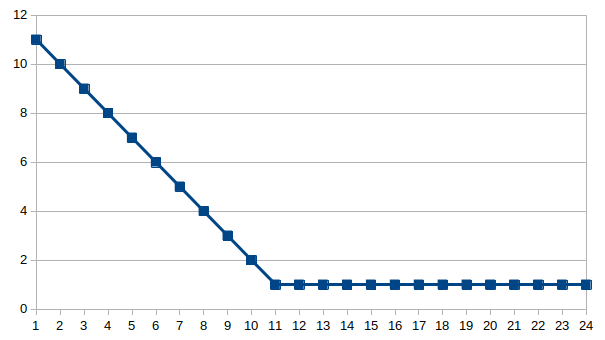
\includegraphics[width=\textwidth]{images/plot_record_perfect.png}
        \caption{Virtual Simulated}
    \end{subfigure}
    ~
    \begin{subfigure}[b]{0.45\textwidth}
        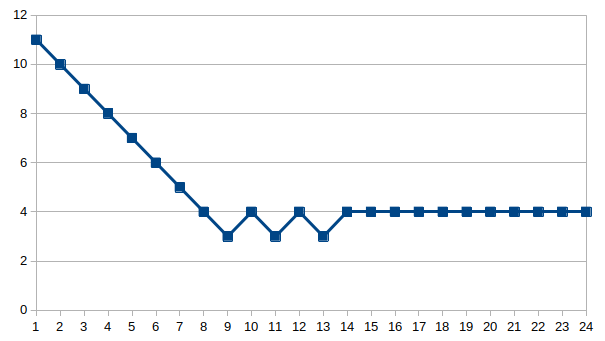
\includegraphics[width=\textwidth]{images/plot_record_normal.png}
        \caption{Normal (test stop at scale 4 or lower)}
    \end{subfigure}
    ~
    \begin{subfigure}[b]{0.45\textwidth}
        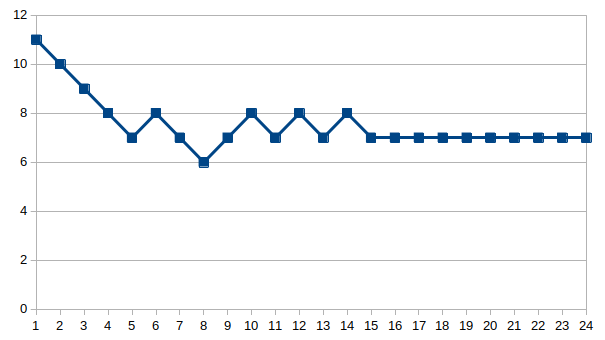
\includegraphics[width=\textwidth]{images/plot_record_mild.png}
        \caption{Not Normal (test stop at scale 7 or higher)}
    \end{subfigure}

    \caption{Example plot of tone-scale record for a tone in each frequency}
\end{figure}


\end{document}




